\chapter{A Gaussian mixture model}\label{ch:gmm}
In \Cref{ch:linear_theory}, we have described a justified framework for computing approximations to the solutions of non-linear SDEs.

When the initial condition is fixed or Gaussian, the resulting linearisation solution is also Gaussian with a mean and covariance that can be computed
A key advantage of the Gaussian solutions the ease of computation; rather than having to generate a large number of realisations of the SDE solution to understand, either qualitatively or for the purposes of inference and estimation, the probability distribution of the solution, we can solve a smaller system of equations \cref{eqn:sigma_def} and for the state and covariance simultaneously.
Even in inference requiring Monte-Carlo simulations, a Gaussian distribution with a specified mean and covariance is faster to sample from than generating numerical solutions of the nonlinear SDE.

An alternative perspective is that the linearisation solution captures the behaviour of stochastic fluctuations close by to a deterministic trajectory, in a similar sense to how a Taylor polynomial captures local behaviour of a nonlinear function.

However, this approximation is only `valid' in the limit of small initial and ongoing uncertainty, which we quantified exactly with the bound in \Cref{thm:main}, and demonstrated heuristically with example SDEs in \Cref{fig:sine_hists,fig:1d_mult_hists,fig:y_hists}.
In practice, the scale of the noise is an inherent part of a model and there is no guarantee that it is sufficiently small for Gaussian approximations to be useful.

We are therfore after a scehme that can produce non-Gaussian approximations to SDE solutions, while still taking advantage of the easy of computation of the corresponding deterministic system and the linearisation approximation.
The lineariusation approximation provides a local understanding of the stochatic solution, and so by `piecing' these approximations together we can capture.
A Gaussian mixture model (GMM) provides a framework for doing exactly this; combining multiple Gaussian densities into a single non-Gaussian distribution.
In this chapter, we outline an algorithm that uses \emph{multiple} Gaussian approximation resulting from the linearised SDE in a mixture model to provide a non-Gaussian approximation to the nonlinear SDE solution.
The algorithm itself is provided in \Cref{sec:gmm_alg}.

The probability density function of a GMM with \(K\) components has the form
\[
	p(z) = \sum_{k=1}^{K}{\omega_i \Gauss{z;\, \mu^{(i)}, \Sigma^{(i)}}},
\]
which consists of \(K\) Gaussian components \(\Gauss{\mu^{(i)}, \Sigma^{(i)}}\) with weights \(\omega_1, \dotsc, \omega_K \geq 0\) satisfying \(\sum_{k=1}^{K}\omega_k = 1\).
\Cref{fig:mixture_model} shows an example of a Gaussian mixture model in 1-dimension with two components; by taking a weighted sum of the \emph{densities}, a non-Gaussian distribution is produced.
With sufficient components, a Gaussian mixture model can recreate any probability distribution in \(\R^n\) while having several of the properties that make Gaussian distributions convenient to work with \citep{McLachlanEtAl_2019_FiniteMixtureModels}.


\begin{figure}
	\begin{center}
		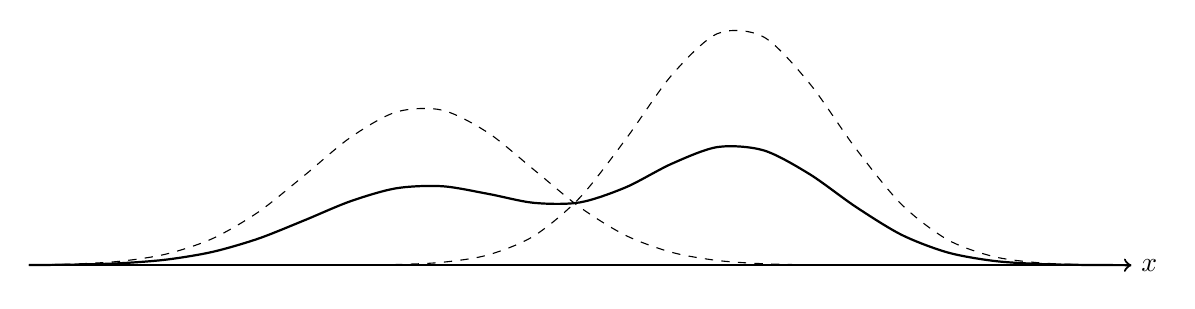
\begin{tikzpicture}
			\draw[scale=2, domain=-3:4, smooth, variable=\x, dashed] plot ({\x}, {exp(-(\x + 0.5) * (\x + 0.5))});
			\draw[scale=2, domain=-3:4, smooth, variable=\x, dashed] plot ({\x}, {1.5*exp(-(\x - 1.5) * (\x - 1.5) / 0.8)});
			\draw[scale=2, domain=-3:4, smooth, variable=\x, thick] plot ({\x}, {0.5 * exp(-(\x + 0.5) * (\x + 0.5)) + 0.5 * 1.5 * exp(-(\x - 1.5) * (\x - 1.5) / 0.8)});
			\draw[->,thick] (-6,0)--(8,0) node[right]{\(x\)};
		\end{tikzpicture}
		\caption{An example of the probability density function of a Gaussian mixture model with two weighted components.
		The two individual components (dashed) are combined to produce the non-Gaussian mixture density (solid).}
		\label{fig:mixture_model}
	\end{center}
\end{figure}


We have a ``local'' approximation for the SDE \cref{eqn:sde_no_eps}, in that solutions to the linearised equation capture the solution behaviour nearby a given deterministic trajectory.
In practice, the solution to stochastic differential equations are non-Gaussian.
A key observation of \Cref{sec:theory_gauss} is that the solution to the linearised SDE is Gaussian when the initial condition is Gaussian.
Through a mixture model, we can capture this non-Gaussianity (leading to a better approximation) while still taking advantage of the computationally efficiency of the Gaussian approximation.

Similar algorithms combining linearisations and mixture models have been proposed, such as that by \citet{DeMarsEtAl_2013_EntropyBasedApproachUncertainty} for propagating an initial uncertainty through a non-linear model, which we compare to.
However, such algorithms have seen little use in practice, particularly in the oceanography and climate modelling circles.
In the following chapter (\Cref{ch:appls}), we will demonstrate the mixture model algorithm on examples from these domains.


\section{Computing the linearised solution distribution}\label{sec:mazzoni}
Prior to detailing our mixture model algorithm, we will first detail a computationally efficient method for computing the
For a Gaussian or fixed initial condition, \Cref{sec:theory_gauss,sec:theory_fixed} respectively established that the solution to the linearised stochastic differential equation is a Gaussian process that is characterised entirely by its mean and covariance matrix.
The computation of this mean and covariance from the model specification is described by \Cref{cor:limit_moments}, and is available as the solution to the joint system:
\td{Ensure notation is consistent!}
\begin{subequations}\label{eqn:gauss_de}
	\begin{align}
		\dod{F_s^t(x)}{t}                & = u\left(F_s^t(x), t\right), \quad F_s^s(x) = x \label{eqn:gauss_mean_de}                                                              \\
		\dod{\Sigma_s^t(x; \Sigma_0)}{t} & = \begin{multlined}[t]
			                                     \nabla u\left(F_s^t(x), t\right) \Sigma_s^t(x; \Sigma_0) + \Sigma_s^t(x; \Sigma_0)\left[\nabla u\left(F_s^t(x), t\right)\right]^{\T} \\
			                                     + \sigma\left(F_s^t(x), t \right)\sigma\left(F_s^t(x), t\right)^{\T},
		                                     \end{multlined}
		\label{eqn:gauss_cov_de}
	\end{align}
\end{subequations}
where \(x\) denotes the initial mean and \(\Sigma_0\) the initial covariance.
To efficiently compute the propagation of a Gaussian uncertainty through the linearised model, as required by our mixture model algorithm, the system \cref{eqn:gauss_de} can be solved jointly subject to the respective initial conditions \(\), where \(x\) here denotes the mean of the initial Gaussian component, and \(\Sigma_0\) the covariance matrix.
Providing that the Jacobian \(\nabla u\) of the vector field is available or can be approximated appropriately, we can propagate each component of the mixture model by solving \cref{eqn:gauss_de}.
An important consideration is that \(\Sigma_s^t\) represents a covariance matrix and must remain symmetric and positive semi-definite when solving \cref{eqn:gauss_de}.
However, many standard numerical ODE schemes do not take this into account, so a specialised scheme is required.
Similar equations of the form \cref{eqn:gauss_de} (although often without dependence on both time and the state in the \(\sigma\) term) are solved numerically in other applications, notably when implementing the extended Kalman filter \citep{Jazwinski_2014_StochasticProcessesFiltering, KulikovaKulikov_2014_AdaptiveODESolvers}.
\citet{KulikovaKulikov_2014_AdaptiveODESolvers} identify that that the two most significant sources of numerical error when solving \cref{eqn:gauss_de} are a) the estimate of the covariance matrix \(\Sigma_s^t\) violating the requirement of positive semi-definiteness, and b) local error propagation in the state equation without an adaptive step size.
Moreover, a computationally efficient algorithm is critical to ensure that our approximate methods have an advantage over bulk Monte-Carlo simulation.

\citet{Mazzoni_2008_ComputationalAspectsContinuous} proposes an efficient hybrid method for solving \cref{eqn:gauss_de} which addresses both difficulties a) and b), and takes advantage of the availability of \(\nabla u\).
This method, which we shall term the Mazzoni method, combines a Taylor-Heun approximation to solve \cref{eqn:gauss_mean_de} for the state and a Gauss-Legendre step to solve \cref{eqn:gauss_cov_de} for the covariance.
With a step size of \(\delta t\), integration for both the state variable and the covariance matrix are convergent with order \(\mathcal{O}\!\left(\delta t^2\right)\).
Moreover, \citet{Mazzoni_2008_ComputationalAspectsContinuous} shows through numerical simulations that the algorithm is computationally efficient when compared to alternatives with moderate precision.
We therefore employ the Mazzoni method for all subsequent implementations of the linearisation procedure, in computing stochastic sensitivity and Gaussian mixture models.

The Mazzoni algorithm is summarised as follows.
Further details on the motivation behind and derivation of these equations is available in the original paper \citep{Mazzoni_2008_ComputationalAspectsContinuous}.
For notational brevity, set \(w_t \equiv F_s^t\!\left(x\right)\) and \(\Pi_t \equiv \Sigma_s^t\!\left(x; \Sigma_0\right)\).
The Taylor-Heun formula for the update of the state over the interval \([t, t + \delta t]\) is then
\begin{subequations}\label{eqn:mazzoni_update}
	\begin{equation}
		w_{t + \delta t} \approx w_t + \left(I - \frac{\delta t}{2}\nabla u\left(w_t, t\right)\right)^{-1}.
		\label{eqn:mazzoni_state_update}
	\end{equation}
	The Gauss-Legendre update of the covariance is
	\begin{equation}
		\Pi_{t + \delta t} \approx M_\tau \Pi_t M_\tau^{\T} + \delta t K_\tau \sigma\left(w_\tau,\, t + \frac{\delta t}{2}\right)\sigma\left(w_\tau,\, t + \frac{\delta t}{2}\right)^{\T} K_\tau^{\T},
		\label{eqn:mazzoni_cov_update}
	\end{equation}
	where
	\begin{align}
		w_\tau & = \frac12\left(w_t + w_{t + \delta t} - \frac{\delta t^2}{4}\nabla u\left(w_t, \, t\right) u\left(w_t, \, t\right)\right) \label{eqn:mazzoni_cov_terms1} \\
		K_\tau & = \left[I - \frac{\delta t}{2}\nabla u\left(w_\tau,\, t + \frac{\delta t}{2}\right)\right]^{-1}                                                          \\
		M_\tau & = K_\tau \left[I + \frac{\delta t}{2}\nabla u\left(w_\tau,\, t + \frac{\delta t}{2}\right)\right] \label{eqn:mazzoni_cov_terms3}.
	\end{align}
	\citet{Mazzoni_2008_ComputationalAspectsContinuous} also provides the option of an adaptive time step to fix the numerical precision while ensuring an computationally efficient algorithm.
	The step size is adjusted by monitoring the error in the estimation of the state variable, aiming to maintain a specified tolerance level \(e > 0\).
	Given the error vector \(\mathcal{E}\) for each component of the state approximation, the maximum total-relative error is
	\begin{equation}\label{eqn:mazzoni_e}
		\hat{e} = \max_{i = 1,\dots,n}\frac{\abs{\mathcal{E}_i}}{\abs{w_{t + \delta t}^{(i)}} + 1}
	\end{equation}
	where \(\mathcal{E}_i\) and \(w_{t + \delta t}^{(i)}\) denote the respective \(i\)th elements of \(\mathcal{E}\) and \(w_{t + \delta t}\), which is used to measure error in the numerical estimate.
	The resulting adjustment factor for the time step is
	\begin{equation}\label{eqn:mazzoni_step}
		\delta t_{\mathrm{new}} = \beta \delta t \sqrt{\frac{e}{\hat{e}}}.
	\end{equation}
	The factor \(\beta\) is a control parameter inserted to avoid frequent recalculations of the step size, and is specified prior.
	\citet{Mazzoni_2008_ComputationalAspectsContinuous} suggests setting \(\beta = 0.8\).
	By again taking advantage of the availability of the Jacobian \(\nabla u\), the error vector is approximated as
	\begin{equation}\label{eqn:mazzoni_err}
		\mathcal{E} \approx \frac{\delta t^2}{2}\left[\frac{1}{3\delta t}\left(\nabla u\!\left(w_{t + \delta t}, t + \delta t\right) - \nabla u\!\left(w_t, t\right)\right) - \frac{1}{6}\nabla u\!\left(w_t, t\right)^2\right] u\!\left(w_t, t\right).
	\end{equation}
\end{subequations}
The set of equations \cref{eqn:mazzoni_update} describe the Mazzoni algorithm, and in \Cref{fig:mazzoni_alg} we summarise the full algorithm, as we have implemented it with adaptive step size.

\begin{figure}
	\begin{center}
		\usetikzlibrary{shapes.geometric, arrows, positioning}

		\begin{tikzpicture}[node distance=70pt]
			\tikzstyle{arrow} = [->,>=stealth]

			\node (s) [rectangle, rounded corners, draw=black, align=center] {\textbf{Start} \\ Given \(s, t, x, \Sigma_0\) \\ Choose \(\delta t_{\mathrm{min}}, \beta, e\)};

			\node (a) [rectangle, below of=s, draw=black, align=center] {Set \(\delta t = \delta t_{\mathrm{min}}\) \\ Set \(k = 0\)};
			\node (b) [rectangle, below of=a, draw=black, align=center] {Set \(t_{k+1} = t_k + \delta t\) \\ Compute \(w_{t_{k+1}}\) with \cref{eqn:mazzoni_state_update} \\
				Compute \(e\) with \cref{eqn:mazzoni_e} \\ Set \(\delta t_{\mathrm{new}} = \max\left\{\delta t_{\mathrm{min}}, \beta \delta t \sqrt{\frac{e}{\hat{e}}}\right\}\)};

			\node (d) [diamond, below of=b, draw=black, align=center, yshift=-40pt] {\(\hat{e} \leq e\) or \\ \(\delta t \leq \delta t_{\mathrm{min}}\)?};
			\node (c) [rectangle, left of=d, draw=black, align=center, xshift=-75pt] {Set \(\delta_t = \delta_{\mathrm{new}}\)};

			\node (e) [rectangle, below of=d, draw=black, align=center, yshift=-20pt] {Compute \(\Pi_{t_{k+1}}\) with \crefrange{eqn:mazzoni_cov_terms1}{eqn:mazzoni_cov_terms3} \\ Set \(k = k + 1\)};

			\node (f) [diamond, below of=e, draw=black, align=center] {\(t_k = T\)?};

			\node (g) [rectangle, rounded corners, left of=f, draw=black, align = center, xshift = -30pt] {\textbf{Stop}};
			\node (h) [rectangle, right of=f, draw=black, align = center, xshift = 75pt] {\(\delta t = \min\left\{\delta t_{\mathrm{new}}, T - t_k\right\}\)};

			\draw [arrow] (s) -- (a);

			\draw [arrow] (a) -- (b);
			\draw [arrow] (b) -- (d);

			\draw [arrow] (d) -- node[anchor=south] {no} (c);
			\draw [arrow] (d) -- node[anchor=east] {yes} (e);

			\draw [arrow] (c) |- (b);

			\draw [arrow] (e) -- (f);

			\draw [arrow] (f) -- node[anchor=south] {yes} (g);
			\draw [arrow] (f) -- node[anchor=south] {no} (h);

			\draw [arrow] (h) |- (b);
		\end{tikzpicture}
		\caption{A flowchart of the Mazzoni algorithm with adaptive time stepping.
			Recreated from Figure 2 of \citet{Mazzoni_2008_ComputationalAspectsContinuous}.}
		\label{fig:mazzoni_alg}
	\end{center}
\end{figure}





\section{The GMM algorithm}\label{sec:gmm_alg}
We now outline the Gaussian mixture model algorithm.

\td{More intuition to explain: can use the component means and covariances to encode uncertainty}

\begin{itemize}
	\item Gaussian distribution captures stochastic variation along a deterministic trajectory - propagate forward until, according to some measure, the Gaussian is no longer a reasonable approximation of the nearby uncertainty.
	\item To capture the non-Gaussianity, we split the Gaussian component into several smaller ones, and then propagate each of these forward.
	\item The component should be split in such a way as to preserve the mean and covariance of the component; a nice property of GMMs is that the overall covariance of the distribution is a sum of the component covariances and the (sample) covariance of the points. Thus, by selecting splitting points that preserve the mean and covariance between themselves, we ensure that the component is not ``lost''.
\end{itemize}


The splitting points should be chosen so that
\begin{equation}
	\frac{1}{K}\sum_{i=1}^K{x^{(k)}} = x, \quad \frac{1}{K}\sum_{i=1}^{K}{\left(x^{(k)} - x\right)\!\left(x^{(k)} - x\right)^{\T}} = \Sigma_0.
	\label{eqn:cov_split_points}
\end{equation}
where the weights \(\)
This ensures that the mean and covariance of the original Gaussian is preserved within the (sample) mean and covariance of the new points themselves.
Note that at least \(K = n + 1\) points are necessary for \cref{eqn:cov_split_points} to be satisfied.
The selection of splitting points are similar to the notion of `sigma points`, employed in the unscented transform to encode an initial mean and covariance \citep{Uhlmann_1995_DynamicMapBuilding,JulierEtAl_2000_NewMethodNonlinear}.
Any such sigma points satisfy \cref{eqn:cov_split_points}---Table I by \citet{MenegazEtAl_2015_SystematizationUnscentedKalman} provides a list of sigma points used across other literature (and reviewed in the context of Kalman filtering)---and therefore can be used in our algorithm.
However, we note a key difference between our proposed algorithm and the unscented transform; \td{what is this difference??}.
The canonical set of sigma points, originally proposed by \citet{Uhlmann_1995_DynamicMapBuilding}, are

which we use to apply the GMM algorithm in \Cref{ch:appls}.
However, we do not enforce a particular approach for selecting these points and leave this to be investigated further as future work.



The Gaussian mixture model is as follows:
\begin{enumerate}
	\item Initialise a Gaussian mixture model with \(N\) components, setting \(t^{(1)} = 0\), \(x^{(1)},\dotsc, x^{(N)}\) to be the component means, \(\Sigma^{(1)}, \dotsc, \Sigma^{(N)}\) to be the component covariance matrices, and \(w^{(1)}, \dotsc, w^{(N)}\) to be the component weights.

	\item While \(t^{(i)} < T\) for any \(i = 1,\dotsc, N\), iterate the following;

	      \begin{enumerate}
		      \item Set \(j\) to be any \(i\) for which \(t^{(i)} < T\).

		      \item Update \(x^{(j)}\) and \(\Sigma^{(j)}\) by solving the joint system \cref{eqn:gauss_approx_des} with initial state \(x^{(j)}\) and covariance \(\Sigma^{(j)}\), terminating when a split condition is met or the final time \(T\) is reached.
		            Denote the time at which this solution terminates as \(t^{(i)}\).

		      \item If \(t = T\), then complete this branch of the algorithm and continue along another branch, if any are still incomplete.

					\item Otherwise, if \(t < T\), construct \(K\) points \(x^{(N + 1)},\dotsc,x^{(N + 2n)}\) that preserve the propagated mean and covariance (i.e. satisfying \cref{eqn:cov_split_points}), setting
		            \[
			            \Sigma^{(N + k)} = \alpha \Sigma^{(1)}, \quad \text{and} \quad w^{(N + k)} = \frac{w^{(1)}}{2n} \quad \text{for each } k = 1,\dotsc,K
		            \]
		            and \(\Sigma^{(1)} = \alpha \Sigma^{(1)}\), \(w^{(1)} = w^{(1)} / K\), and \(N = N + K\).
	      \end{enumerate}

	\item Construct the mixture model with density function
	      \[
		      G\left(x\right) = \frac{1}{\sum_{l=1}^{N}w^{(l)}}\sum_{i=1}^{N}{w^{(i)}\Gauss{x; \, x^{(i)}, \Sigma^{(i)}}}.
	      \]

\end{enumerate}
Note that we have presented a general framework, with several choices for specific implementations left unfulfilled.

There are several options for initialising the mixture model, depending on the initial condition.
For a fixed initial condition \(x_0\), we can take the degenerate mixture model with a single component and zero variance, i.e.
\[
	N = 1, \quad x^{(1)} = x_0, \quad \Sigma^{(1)} = O, \quad w^{(1)} = 1.
\]



\Cref{fig:gmm_steps} provides a pictorial representation of the propagation and splitting of a single component in the mixture model.


\begin{figure}
	\captionsetup{singlelinecheck=off}
	\begin{center}
				\begin{tikzpicture}
				\draw (-1,5) node {1)};
				% STEP 0: INITIAL
				% Initial position
				\fill[black] (1,2.5) circle[radius=1pt] node[anchor = east] {\(x\)};

				% Initial covariance
				\draw[dashed, rotate around = {58: (1, 2.5)}, blue] (1,2.5) ellipse (14pt and 22pt);
				\node[blue] at ($(1,2.5)+(90:14pt and 22pt)$) {\(\Sigma_0\)};

				% STEP 1: PROPAGATE
				\draw (6,5) node {2)};
				% Trajectory
				\draw (7,2.5) .. controls (9,4.5) and (11,-0.5) .. (13,2.5);

				% Initial position
				\fill[black] (7,2.5) circle[radius=1pt] node[anchor = east] {\(x\)};

				% Initial covariance
				\draw[dashed, rotate around = {58: (7, 2.5)}, gray] (7,2.5) ellipse (14pt and 22pt);

				% Mapped position
				\fill[black] (13,2.5) circle[radius=1pt] node[anchor = south] {\(F_0^t\!\left(x\right)\)};

				% Covariance ellipse
				\draw[dashed, rotate around = {30: (13,2.5)}, red] (13,2.5) ellipse (30pt and 70pt);
				% \draw[dashed, rotate around = {30: (8,0)}, red] (8,0) ellipse (20pt and 50pt);
				% \draw[dashed, rotate around = {30: (8,0)}, red] (8,0) ellipse (10pt and 30pt);
				\node[red] at ($(13,2.5)+(75:30pt and 70pt)$) {\(\Sigma_0^t\!\left(x\right)\)};

				% STEP 2: Splitting
				\draw (-1, -1) node {3)};
				% Trajectory
				\draw[gray] (1,-5) .. controls (3,-3) and (5,-8) .. (7,-5);

				% Initial position
				\fill[gray] (1,-5) circle[radius=1pt] node[anchor = east] {\(x\)};

				% Mapped position
				\fill[blue] (6,-5) circle[radius=1pt];

				% Covariance ellipse
					\draw[dashed, rotate around = {30: (6,-5)}, gray] (6,-5) ellipse (30pt and 70pt);

				% Additional sigma points
				\fill[blue, rotate around = {30: (6,-5)}] ($(6, -5)+(0:30pt and 70pt)$) circle[radius=1pt];
				\fill[blue, rotate around = {30: (6,-5)}] ($(6, -5)+(90:30pt and 70pt)$) circle[radius=1pt];
					\fill[blue, rotate around = {30: (6,-5)}] ($(6, -5)+(180:30pt and 70pt)$) circle[radius=1pt];
				\fill[blue, rotate around = {30: (6,-5)}] ($(6, -5)+(270:30pt and 70pt)$) circle[radius=1pt];

				% Covariances for each sigma point
				\draw[dashed, rotate around = {30: (6,-5)}, blue] (6, -5) ellipse (12pt and 28pt);
				\draw[dashed, rotate around = {30: (6,-5)}, blue] ($(6, -5)+(0:30pt and 70pt)$) ellipse (12pt and 28pt);
				\draw[dashed, rotate around = {30: (6,-5)}, blue] ($(6, -5)+(90:30pt and 70pt)$) ellipse (12pt and 28pt);
				\draw[dashed, rotate around = {30: (6,-5)}, blue] ($(6, -5)+(180:30pt and 70pt)$) ellipse (12pt and 28pt);
				\draw[dashed, rotate around = {30: (6,-5)}, blue] ($(6, -5)+(270:30pt and 70pt)$) ellipse (12pt and 28pt);

					% STEP 3: Continued propagation
					\draw (4, 0) node {4)};
					\fill[blue] (11,-5) circle[radius=1pt];

					% Additional sigma points
					\fill[blue, rotate around = {30: (11,-5)}] ($(11,-5)+(0:30pt and 70pt)$) circle[radius=1pt];
					\fill[blue, rotate around = {30: (11,-5)}] ($(11,-5)+(90:30pt and 70pt)$) circle[radius=1pt];
					\fill[blue, rotate around = {30: (11,-5)}] ($(11,-5)+(180:30pt and 70pt)$) circle[radius=1pt];
					\fill[blue, rotate around = {30: (11,-5)}] ($(11,-5)+(270:30pt and 70pt)$) circle[radius=1pt];

					% Covariances for each sigma point
					\draw[dashed, rotate around = {30: (11,-5)}, gray] (11,-5) ellipse (12pt and 28pt);
					\draw[dashed, rotate around = {30: (11,-5)}, gray] ($(11,-5)+(0:30pt and 70pt)$) ellipse (12pt and 28pt);
					\draw[dashed, rotate around = {30: (11,-5)}, gray] ($(11,-5)+(90:30pt and 70pt)$) ellipse (12pt and 28pt);
					\draw[dashed, rotate around = {30: (11,-5)}, gray] ($(11,-5)+(180:30pt and 70pt)$) ellipse (12pt and 28pt);
					\draw[dashed, rotate around = {30: (11,-5)}, gray] ($(11,-5)+(270:30pt and 70pt)$) ellipse (12pt and 28pt);

					% New trajectories
					% \draw[black, rotate around = {30: (6,0)}] (6, 0) .. controls (8, -2) and (9, 0.8) .. (12, -1);
					\draw[black, rotate around = {30: (11,-5)}] ($(11,-5)+(0:30pt and 70pt)$) .. controls (13, -4.5) and (14, -4.2) .. (16.5, -5.3);
					\draw[black, rotate around = {30: (11,-5)}] ($(11,-5)+(90:30pt and 70pt)$) .. controls (13, -5) and (15, -6.2)  .. (17.7, -6);
					% \draw[black, rotate around = {30: (6,0)}] ($(6, 0)+(180:30pt and 70pt)$) .. controls (8, -2) and (9, 0.8) .. (12, -2);
					% \draw[black, rotate around = {30: (6,0)}] ($(6, 0)+(270:30pt and 70pt)$) .. controls (8, -2) and (9, 0.8) .. (12.2, 0.6);

			\end{tikzpicture}
		\caption[The propagation and splitting of a component in the Gaussian mixture model:]{The propagation and splitting of a component in the Gaussian mixture model:
		\begin{enumerate*}
			\item Start with the mean \(x\) and covariance matrix \(\Sigma_0\) for a component of the mixture model.
			\item The mean \(x\) and covariance matrix \(\Sigma_0\) of the component are propagated forward through the linearised SDE, by solving \cref{eqn:gauss_de}.
			\item Once the splitting criterion is met, the covariance matrix is split into \(K\) smaller covariance matrices, with corresponding means so that the mean and covariance of the propagated point is preserved.
			\item Each new component is propagated forward with \cref{eqn:gauss_de} and the process is repeated for each component \emph{individually} until the final time is reached.
		\end{enumerate*}}
		\label{fig:gmm_steps}
	\end{center}
\end{figure}


\section{Error remains bounded}
Our main result of \Cref{ch:linear_theory}, \Cref{thm:main}, establishes that the strong error in approximating the solution to a small-noise nonlinear stochastic differential equation with a linearisation is bounded by a scaling of the initial and ongoing uncertainty scales.
In this section, we show that this result implies that if we propagate the components of a Gaussian mixture model with linearisations about the component means, as our mixture model algorithm employs, the error remains bounded in a similar fashion.

Recall the results of \Cref{sec:theory_gauss}, the SDE linearisation theory applied to the special case of a Gaussian initial condition.
Suppose that \cref{eqn:sde_no_eps} is subject to a Gaussian initial condition \(x \isGauss{\mu_0, \delta^2\Sigma_0}\), where \(\mu_0 \in \R^n\) and \(\Sigma_0 \in \R^{n\times n}\) are fixed and \(\delta > 0\) is a scaling parameter.
We can linearise \cref{eqn:sde_no_eps} about the deterministic trajectory \(F_t^0\!\left(\mu_0\right)\) originating from the mean \(\mu_0\), as
\begin{equation}
	\dif l_t\!\left(\mu_0, \delta^2\Sigma_0\right) = \begin{multlined}[t]
		\left[F_0^t\!\left(\mu_0\right) + \nabla u\!\left(F_0^t\!\left(\mu_0\right), t\right)\left(l_t\!\left(\mu_0, \delta^2 \Sigma_0\right) - F_0^t\!\left(\mu_0\right)\right)\right]\dif t \\
		+ \epsilon\sigma\!\left(F_0^t\!\left(\mu_0\right), t\right)\dif W_t, \quad l\!\left(\mu_0, \delta^2\Sigma_0\right) = x.
	\end{multlined}
	\label{eqn:scaled_sde_linear}
\end{equation}
We have introduced the notation \(l_t\!\left(\mu_0, \delta^2\Sigma_0\right)\) to indicate the dependence of the linearised solution on the initial mean and covariance matrix.
The solution to \cref{eqn:scaled_sde_linear} at time \(t\) follows a Gaussian distribution with computable mean and covariance, specifically
\[
	l_t\!\left(\mu, \delta^2\Sigma_0\right) \isGauss{F_0^t\!\left(\mu_0\right), \, \delta^2 \nabla F_0^t\!\left(\mu_0\right) \Sigma_0 \left[\nabla F_0^t\!\left(\mu_0\right)\right]^{\T} + \epsilon^2\Sigma_0^t\!\left(\mu_0\right)},
\]
where
\[
	\Sigma_0^t\!\left(\mu_0\right) = \nabla F_0^t\!\left(\mu_0\right)\int_0^t{\left[\nabla F_0^\tau\!\left(\mu_0\right)\right]^{-1} \sigma\!\left(F_0^\tau\!\left(\mu_0\right), \tau\right)\sigma\!\left(F_0^\tau\!\left(\mu_0\right), \tau\right)^{\T}\left[\nabla F_0^\tau\!\left(\mu_0\right)\right]^{^{-\intercal}}\dif\tau}\left[\nabla F_0^t\!\left(\mu_0\right)\right]^{\T}.
\]
\Cref{thm:main} establishes that for any \(t \in [0,T]\), there exists constants \(A_1(t), A_2(t), A_3(t) \geq 0\) independent of \(\mu_0\) such that
\begin{equation}\label{eqn:linear_error_bound}
	\avg{\norm{y_t - l_t\!\left(\mu_0, \delta^2 \Sigma_0\right)}} \leq A_1(t)\epsilon^2 + A_2(t)\epsilon\delta + A_3(t)\delta^2.
\end{equation}
Note that we have dropped the notation indicating the dependence of the constants on the coefficient bounds for notational brevity.
For completeness, however, we have
\begin{align*}
	A_1(t) & = \left(K_{\nabla\nabla u} + K_{\nabla\sigma}\right)D_1\!\left(1, t, K_{\nabla u}, K_\sigma\right) \\
	A_2(t) & = K_{\nabla\nabla u} D_2\!\left(1, t, K_{\nabla u}\right)                                          \\
	A_3(t) & = K_{\nabla\sigma}D_3\!\left(1, t, K_{\nabla u}\right),
\end{align*}
using the notation of \Cref{thm:main}.
Suppose at a time \(s \in [0,T]\), we have a mixture model with \(M\) Gaussian components
\[
	p_0\!\left(z\right) = \sum_{i=1}^{M}{\omega_i\Gauss{z;\, \mu_0^{(i)}, \delta^2\Sigma_0^{(i)}}}
\]
where \(\omega_1,\dotsc, \omega_M \geq 1\) are weights satisfying \(\sum_{i=1}^M{\omega_i} = 1\), \(\mu_0^{(1)}, \dots \mu_0^{(M)}\) are the component means and \(\Sigma_0^{(1)}, \dotsc, \Sigma_0^{(M)}\) are the component covariance matrices.
Via linearisation approximations of the form \cref{eqn:scaled_sde_linear}, we construct the mixture model at time \(t > s\)
\[
	p_t\!\left(z\right) = \sum_{i=1}^{M}{\omega_i\Gauss{z; \, F_s^t\!\left(\mu_0^{(i)}\right), \Pi^{(i)}}},
\]
where
\[
	\Pi^{(i)} = \delta^2 \nabla F_0^t\!\left(\mu_0\right) \Sigma_0^{(i)} \left[\nabla F_s^t\!\left(\mu_0\right)\right]^{\T} + \epsilon^2 \Sigma_s^t\!\left(\mu_0\right),
\]
is the propagated covariance matrix.
Let \(\Xi_0\) be a random variable distribution distributed according to \(p_0\), which we can write as
\[
	\Xi_0 = \sum_{i=1}^{M}{I_i \xi_0^{(i)}}
\]
where \(\xi_0^{(i)} \isGauss{\mu_0^{(i)}, \Sigma_0^{(i)}}\) independently for each \(i\), and \(\left(I_1, \dotsc, I_M\right)\) are a set of indicator variables with
\[
	P\!\left(I_i = 1,\, I_j = 0 \text{ for all } j \neq i\right) = \omega_i,
\]
for each \(i = 1,\hdots,M\), and zero probability otherwise.
Similarly, let \(\Xi_t\) be a random variable distributed according the mixture model \(p_t\), which we construct from solutions to linearised SDEs of the form \cref{eqn:scaled_sde_linear}, by writing
\[
	\Xi_t = \sum_{i=1}^{M}{I_i l_t\!\left(\mu_0^{(i)}, \delta^2\Sigma_0^{(i)}\right)},
\]
where each solution to \cref{eqn:scaled_sde_linear} is independent of the others.
Then, for any \(i\) we have the conditional distribution
\[
	\left. \Xi_t \, | \, \set{I_i = 1, \, I_j = 0 \text{ for all } j \neq i} \right. = l_{t}\left(\mu_0^{(i)}, \delta^2 \Sigma_0^{(i)}\right).
\]
The random variable \(\Xi_t\) represents our approximation of the state at time \(t\), after a single step of the mixture model algorithm.
Via the law of total expectation, the error in approximating \(y_t\) with \(\Xi_t\) is
\begin{align*}
	\avg{\norm{y_t - \Xi_t}} & = \sum_{i=1}^{M}{\avg{\norm{y_t - \Xi_t}\,\middle|\, I_i = 1}}P\!\left(I_i = 1,\, I_j = 0 \text{ for all } j \neq i\right) \\
	                         & = \sum_{i=1}^{M}{\omega_i\avg{\norm{y_t - l_{t}\left(\mu_0^{(i)}, \delta^2 \Sigma_0^{(i)}\right)}}}                        \\
	                         & = \sum_{i=1}^{M}{\omega_i\left(A_1(t)\epsilon^2 + A_2(t) \epsilon \delta + A_3(t)\delta^2\right)}                          \\
	                         & = A_1(t) \epsilon^2 + A_2(t)\epsilon\delta + A_3(t)\delta^2.
\end{align*}
In the mixture model algorithm described, the initialising uncertainty (being a component of the mixture model) at each step scales with \(\epsilon\), specifically \(\delta = \epsilon\).
Thus, the error in the algorithm remains bounded with order \(\epsilon^2\).


\section{The splitting criterion}
The mixture model described in \Cref{sec:gmm_alg} requires a choice of criterion for when to split a Gaussian component, for which there are several choices.
A given Gaussian component should be split when the linearised SDE is no longer a reasonable approximation for the original SDE about the deterministic trajectory corresponding to the component.



\citet{DeMarsEtAl_2013_EntropyBasedApproachUncertainty} propose an algorithm for propagating an initial uncertainty through a nonlinear model, by using a Gaussian mixture model and a similar splitting algorithm.
... The sigma point method provides an \emph{exact} computation for the covariance matrix of a deterministic nonlinear transformation of a random variable.

% \section{Analysis through exact SDE solutions}

% To examine the performance of the mixture model algorithm, in producing an approximate density solution to a stochastic differential equation, as to justify the choices of the heuristics involved, we shall consider three simple examples.
% These examples, two of which are in one-dimension, have weak solutions with probability density functions which can be derived analytically, and therefore provide us with a ``ground truth'' to compare to which is otherwise missing from the applications we are interested in.
% Our three examples were introduced and detailed in \Cref{sec:back_sde_solutions}.


% \subsection{A linear SDE}
% Consider an \(n\)-dimensional linear stochastic differential equation with additive noise;
% \begin{equation}
% 	\sde{y_t}{A(t)y_t}{B(t)},
% 	\label{eqn:linear_n_sde}
% \end{equation}
% where \(A: [0,T] \to \R^{n\times n}\) and \(B: [0,T] \to \R^{n \times m}\) are specified, deterministic matrix-valued functions that are sufficiently smooth and measurable to ensure the existence of solutions, and \(W_t\) is an \(m\)-dimensional Wiener process.

% At time \(t \in [0,T]\),
% \[
% 	y_t \isGauss{\exp\left[\int_0^{t}{A(\tau)\dif \tau}\right]y_0, \, },
% \]\td{Calculate properly}
% where \(\exp\left[\cdot\right]\) here denotes the matrix exponential.
% For this SDE, the Gaussian approximation \cref{eqn:sde_gauss_approx_no_epsilon} is therefore exact, in that it describes exactly the time-marginal distribution of the solution.
% In our mixture model framework, there is hence no need to place down any covariance-preserving points; for a fixed initial condition, a single Gaussian computed about the deterministic trajectory emanating from that point is sufficient.
% Hence, as a ``sanity check'' we would expect that our mixture model algorithm recognises that model is linear and the condition for placing covariance-preserving points is not reached.





% \subsection{Ben\^e's SDE}


% \subsection{Linear dynamics and multiplicative noise}



% \section{StochasticSensitivity.jl}
